
\documentclass[10pt,journal,compsoc]{styles/IEEEtran}
\usepackage{styles/algorithm}
\usepackage[noend]{styles/algorithmic}
\usepackage{graphicx}
\usepackage{color}
\usepackage{listings}
\usepackage{amsmath}
\usepackage[utf8]{inputenc}
\usepackage[T1]{fontenc}
\usepackage[labelformat=empty]{caption}
% *** CITATION PACKAGES ***
\ifCLASSOPTIONcompsoc
  % IEEE Computer Society needs nocompress option
  % requires cite.sty v4.0 or later (November 2003)
  \usepackage[noadjust]{cite}
\else
  % normal IEEE
  \usepackage{cite}
\fi

\title{Tarea 3: MÉTODO DE GRADIENTE CONJUGADO}

\author{Juan Gerardo Fuentes Almeida}

% The paper headers
\markboth{Tarea 3 MÉTODO DE GRADIENTE CONJUGADO}%
{Shell \MakeLowercase{\textit{et al.}}: Bare Advanced Demo of styles/IEEEtran.cls for Journals}

\IEEEtitleabstractindextext{%
\begin{abstract}
En esta pr\'actica se implementa el algoritmo de Gradiente Conjugado en un problema de regularizaci\'on de imágenes. Asimismo se hacen comparaciones en tiempo e iteraciones con el método de Gauss-Seidel.
\end{abstract}
}

\begin{document}

% make the title area
\maketitle

\IEEEdisplaynontitleabstractindextext

\IEEEpeerreviewmaketitle

\section{Introducci\'on}

\IEEEPARstart{L}os métodos de Gradiente Conjugado se encuentran entre los mas útiles para resolver sistemas grandes de ecuaciones, no requieren almacenamiento de matrices y nos permiten resolver problemas de optimización cuadrática.\\

La forma lineal del método de Gradiente Conjugado consiste en un método iterativo para resolver sistemas lineales con matrices definidas positivas. Su desempeño esta determinado por la distribución de los eigenvalores de la matriz, esta distribución se puede trasformar o pre-condicionar para mejorar significativamente la convergencia del método.
 
\section{Teoría}

\subsection{Gradiente Conjugado Lineal}

Se utiliza para resolver sistemas de ecuaciones lineales de la forma $Ax=b$ para $A$ simétrica positiva definida, se resuelve el problema de minimización\\

min $\phi (x)=\frac{1}{2} x^T A x-b^T x$\\

El gradiente $\nabla \phi(x)$ equivale al residuo del sistema lineal\\

$\nabla \phi (x) = Ax-b = r(x)$\\

para una particular $x=x_k$ se tiene $r_k=Ax_k-b$\\

\subsubsection{Métodos de Dirección Conjugada}

Los métodos de dirección conjugada se caracterizan por poder generar conjunto de vectores no nulos ${p_0,p_1,...,p_n}$ tales que para una matriz simétrica y positiva definida $A$ se tiene que\\

$p_i^T A p_j=0 \forall i\neq j$\\

se dice entonces que estos vectores son \emph{conjugados} respecto a la matriz $A$\\

La importancia de esto es que podemos minimizar $\phi$ en n pasos minimizando sucesivamente a lo largo de direcciones individuales en un conjunto conjugado. Dado un punto de inicio $x_0$ y un conjunto de direcciones conjugadas, podemos establecer la secuencia\\

$x_{k+1}=x_k+\alpha_k p_k$\\

donde $\alpha_k$ es el minimizador de la función $\phi$ determinada explícitamente por

$\alpha_k=-\frac{g_k^T p_k}{p_k^T A p_k}$

\begin{figure}[hbtp]
\centering
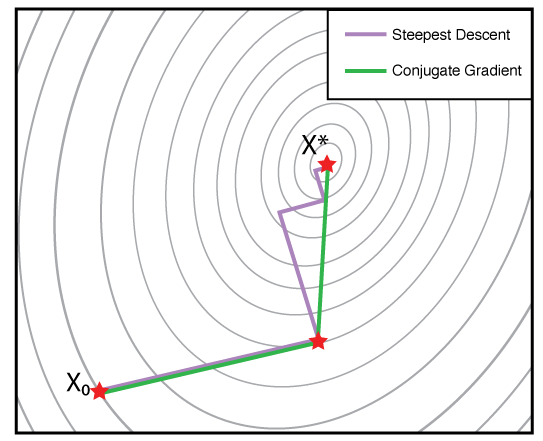
\includegraphics[width=0.45\textwidth]{conjugateGradient.png}
\caption{Dirección del Gradiente Conjugado}
\end{figure}
 
En el método de Gradiente Conjugado, cada dirección $p_k$ se elige como una combinación lineal del residuo negativo $-r_k$, el cual es la dirección de máximo descenso para la función $\phi$, y la dirección anterior $p_{k-1}$\\

$p_k=-g_k+\beta_k p_{k-1}$\\

donde el escalar $\beta_k$ se determina de forma que $p_k$ y $p_{k-1}$ sean conjugados respecto a $A$:\\

$\beta_k=\frac{g_k^T A p_{k-1}}{p_{k-1}^T A p_{k-1}}$\\

En esta pr\'actica calculamos $\beta_k$ de acuerdo a la definición de Fletcher-Reeves:\\

$\beta_k=\frac{g_k^T g_k}{g_{k-1}^T g_{k-1}}$\\




 
\section{Resultados}

Como parte de la pr\'actica, se tom\'o un conjunto de im\'agenes de resonancia magn\'etica para implementar un registro r\'igido y minimizar la funci\'on de error determinada por la siguiente expresi\'on:\\

\begin{figure}[hbtp]
\centering
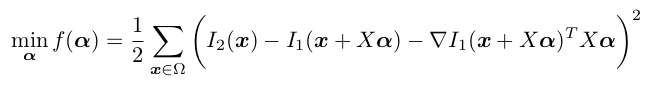
\includegraphics[width=0.45\textwidth]{error.png}
\caption*{}
\end{figure}

$I_2$ es una imagen de referencia, $I_1$ es la imagen observada cuyo dominio est\'a definido en $x={x_1,x_2}$, de manera que $\omega$ representa el conjunto de todos los pixeles de la imagen, $X$ y $\alpha$ son variables definidas de la siguiente manera:\\

\begin{figure}[hbtp]
\centering
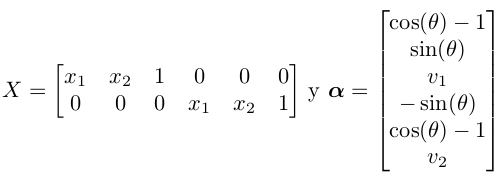
\includegraphics[width=0.45\textwidth]{variable.png}
\caption*{}
\end{figure}

Esto permite que la transformaci\'on de una imagen a otra este dada por el producto $x+X\alpha$\\


\begin{figure}[hbtp]
\centering
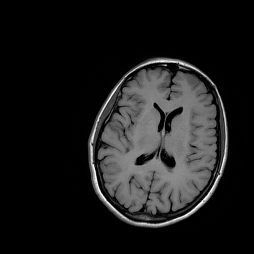
\includegraphics[width=0.35\textwidth]{mriC.png}
\caption{Imagen Inicial u Observada}
\end{figure}

\begin{figure}[hbtp]
\centering
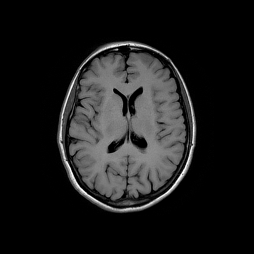
\includegraphics[width=0.35\textwidth]{mriReferencia.png}
\caption{Imagen de referencia}
\end{figure}

El gradiente y el Hessiano de esta funci\'on est\'an definidos de la siguiente manera:\\

$\nabla f(\alpha)=\Sigma[I_2(x)-I_1(x)][-X^T \nabla I_1(x+X\alpha)]$\\
$\nabla^2 f(\alpha)=\Sigma[X^T \nabla I_1(x+X\alpha)][X^T \nabla I_1(x+X\alpha)]^T$\\

En la pr\'actica, estas funciones fueron las que nos dieron mejores resultados.\\

El algoritmo lee los archivos de las dos im\'agenes y realiza la minimizaci\'on de la funci\'on objetivo con el m\'etodo de la Regi\'on de Confianza, en conjunto con el m\'etodo de Dogleg para el c\'alculo del punto de Cauchy; se inicia con un desplazamiento inicial de 10 pixeles hacia arriba y hacia la izquierda para acercarnos un poco a la posici\'on de la imagen de referencia.

\begin{figure}[hbtp]
\centering
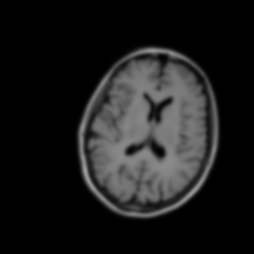
\includegraphics[width=0.35\textwidth]{mriCinicial.png}
\caption{Imagen inicial, se tuvo que hacer un emborronado de la imagen para obtener mejores resultados}
\end{figure}

\begin{figure}[hbtp]
\centering
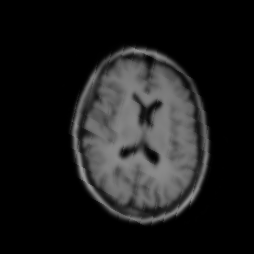
\includegraphics[width=0.35\textwidth]{mriCfinal.png}
\caption{Imagen final despues de 20 mejoras, se aprecia la rotacion que se produce para empalmarse con la imagen de referencia}
\end{figure}

Aunque la funci\'on objetivo siempre muestra valores demasiado grandes, se pudo observar una mejor\'ia en la posici\'on y orientaci\'on de la imagen con respecto a la de referencia. Otro comportamiento observado fue que a partir de cierto n\'umero de iteraciones, la funci\'on objetivo deja de disminuir qued\'andose en un valor muy grande y reduciendo pr\'acticamente a cero la regi\'on de confianza.


\section{Conclusiones}

En general no se obtuvieron los resultados que se esperaban, se tuvieron muchos problemas, principalmente con repecto a la correcta definici\'on de la funci\'on objetivo y sus derivadas, tambi\'en se tuvieron problemas con los m\'etodos de optimizaci\'on vistos en clase, los cuales directamente aplicados a este problema no produc\'ian los resultados esperados. Se espera que en futuras pr\'acticas se afinen m\'as detalles sobre este tipo de implementaciones.

\bibliographystyle{plain}
\bibliography{biblio}


\appendix
\section{Implementation details}
El programa est\'a implementado tomando en cuenta todas estandarizaciones indicadas en el curso.

Un \textit{makefile} ha sido generado, el cual soporta los comandos \textit{make}, \textit{run} and \textit{clean}. El programa recibe como primer argumento el nombre del archivo de la imagen inicial, y como segundo argumento el nombre del archivo de la imagen de referencia.


\end{document}


